\chapter{Introduction}

\begin{sloppypar}
The mountainous Zagros regions of northwestern Iran and northern Iraq are characterised by rich linguistic diversity. Varieties of Kurdish\il{Kurdish} are spoken across much of the area, along with remaining varieties of Gorani\il{Gorani} and Neo-Aramaic\il{Neo-Aramaic}. Over the last two decades, there has been a growing interest in documenting peripheral Gorani\il{Gorani} varieties, leading to the publication of a few sketch grammars of these endangered languages (see \citeauthor{mahmoudveysi_gorani_2012}'s \citeyear{mahmoudveysi_gorani_2012} description of the Gewrecû\il{Gorani!Gewrecû} variety, \citeauthor{mahmoudveysi_gorani_2013}'s \citeyear{mahmoudveysi_gorani_2013} description of the Zerde\il{Gorani!Zerde} variety). Despite these welcome documentation efforts, the more conservative Hewramî\il{Hewramî} varieties of Gorani\il{Gorani} have lacked a decent monograph-length description since \citegen{mackenzie_dialect_1966} seminal sketch grammar of the Luhon variety of Hewram\^i\il{Hewramî!Luhon}. 

This book aims to fill this gap by providing a comprehensive grammar of the Tekht variety of Hewramî\il{Hewramî!Tekht}, one of the most conservative Hewramî\il{Hewramî} varieties spoken in the high mountainous region of Hewraman Tekht straddling Iranian and Iraqi Kurdistan. The grammar is accompanied by a Hewramî\il{Hewramî}-English\il{English} glossary, an English\il{English}-Hewramî\il{Hewramî} glossary, and a verb list. 

This chapter is structured as follows: \S\ref{Hew-dialects} provides a general description of Hewramî\il{Hewramî} and its varieties. \S\ref{sect:hew.ir.dialectology} discusses the place of Hewramî\il{Hewramî} within Iranian languages. Then, I move on to give a brief description of Hewraman Tekht (\S\ref{sect:hewramitext}), followed by the affiliation of the Tekht variety within Hewramî\il{Hewramî} dialectology (\S\ref{sect:affiliation-hew}). In \S\ref{sect:lit.gorani}, I give an overview of the literature on Gorani\il{Gorani} varieties. \S\ref{sect:fieldwork} summarises the fieldwork behind producing this grammar. The chapter ends with information about the main corpus of narrative texts (\S\ref{sect:corpus.hewrami-text}) behind this study, followed by an additional corpus of folktales used to back up the description of morphosyntactic features (\S\ref{sect:folktale-corpus}).


\section{Hewramî\il{Hewramî} and its varieties}\label{Hew-dialects}

Hewramî\il{Hewramî} is an Iranian language spoken in the remote mountainous region at the heart of the Kurdish\il{Kurdish}-speaking region along the western border of Iran and neighbouring areas in Iraqi Kurdistan. Hewramî\il{Hewramî} is a name used by Hewramî\il{Hewramî} people to refer to themselves and their language. Published references to the language appear in the following forms: Awromānie\il{Hewramî} \citep{christensen_les_1921}; Auramânî\il{Hewramî} \citep{mann_mundarten_1930}; Hawrāmī\il{Hewramî} \citep{mackenzie_dialect_1966,mahmoudveysi_hawrami_2018}; Hawrami\il{Hewramî} \citep{karimi_noun_2008, haig_alignment_2008, stilo_loss_2019}. The exonyms \textit{maço} `he/she says' and \textit{maço zuwan} `maço language' are sometimes used by neighbouring Kurdish\il{Kurdish}-speaking people to refer to the language. In addition, in some linguistic studies, e.g., Khan \& Mohammadirad (\citeyear{khan_language_2023}, \citeyear{KhanMohammadirad+2024+171+198}), the cover term Gorani\il{Gorani} has been used interchangeably with Hewramî\il{Hewramî}. 

\citet{MacKenzie1987Avroman} classifies the Hewraman region into four main divisions: Luhon (in the south), Tekht (in the centre), Dizlî (in the north), and Razaw (around Sarv Abad). The last one could include the Jawero and Gawero sub-regions \citep{mahmoudveysi_hawrami_2018}.\footnote{It has yet to be determined whether these geographical divisions match linguistic subdivisions, especially in the Dizlî and Razaw regions.} Hewramî\il{Hewramî} varieties are traditionally divided into three major groupings: Tekht, Luhon, and Jawero. Geographically speaking, these varieties are spoken in the centre, south, and east of the greater Hewraman region, respectively. The Tekht region is linked to Jawero through a stretch of valleys, while the Luhon region is located in the western valley. Within Iran, the most significant concentration of Hewramî\il{Hewramî} speakers is in the cities of Mariwan, Pawa, and Sarv Abad, though Kurdish\il{Kurdish} is also spoken in these three cities. In Iraqi Kurdistan, Hewramî\il{Hewramî} speakers can be found in cities such as Khurmal and Halabja. Figure \ref{fig:hewmap} shows the region of Hewraman according to the mentioned divisions.\footnote{The villages in each part are as follows. The local name has appeared in the Latin Kurdish\il{Kurdish} alphabet for each locality, followed by the official name in the transcription common in Iranian philology. The localities in Iraqi Kurdistan have been transcribed only in the Kurdish\il{Kurdish} alphabet. \\
\textbf{Dizlî region}: (1) Dizɫî (Dezli); (2) Qeɫacê (Qal'eh Ji); (3) Baramawa (Bahrām Ābād); (4) Tifɫî (Tefli); (5) Tazawa (Tāzeh Ābād); (6) Bindoɫ (Bendowl); (7) Deymeyo (Demayo); (8) Derokî (Daraki); (9) Gorgeyî (Ebrāhim Ābād); (10) Zelke (Zalkeh); (11) Dere (Darreh); (12) Zeɫm; (13) Ehmewawa; (14) Hanew Qulî. \\
\textbf{Tekht region}: (1) Hewraman Tekht (Owrāmān Takht); (2) Weysîyan (Veysiān); (3) Biɫbeř (Belbar); (4) Serû Pîrî (Sar Pir); (5) Jîwar (Zhivār); (6) Silên (Selin); (7) Espeřêz (Aspeh Riz); (8) Del (Dal); (9) Nwên (Nevin); (10) Kelcî (Kalji); (11) Naw (Nav); (12) Daɫemerz (Daleh marz); (13) Zom (Zom); (14) Kemaɫe (Kamāleh); (15) Bennen (Bannan); (16) Wergewîyare (Vargeh Vir); (17) Rûwar (Ruvār); (18) Hewasawa (Abbās Ābād). \\
\textbf{Luhon region}: (1) Nođşe (Nodsheh); (2) Newsû (Nowsud); (3) Pawe (Pāveh); (4) Keymne (Keymneh); (5) Zawer (Zāvar); (6) Hane Geřmeɫe (Hāneh Garmaleh); (7) Hecîc (Hajij); (8) Nerwe (Narveh); (9) \c{S}oşme (Shushmeh); (10) \c{S}êxan (Sheykhān); (11) Xaneqa (Khaneqā); (12) Deremûr (Darreh Mur); (13) Giraɫ (Gerāl); (14) Neysane (Naysāneh); (15) Sosekan; (16) Tewêɫe; (17) Bîyare; (18) Baxe Kon; (19) Serget; (20) Dere Mar; (21) Gulp; (22) Dega \c{S}êxan. \\
\textbf{Razaw region}: (1) \v{R}azaw (Raz Āb); (2) Keřawa (Karr Ābād); (3) Degaga (Degāgāh); (4) Dêweznaw (Divaz Nāv); (5) Coɫandê (Jowlān Deh); (6) Nawe (Nāveh); (7) Xaneqay \v{R}azaw (Khāneqāhe Raz Āb); (8) Dořû (Dorud); (9) Mehmûawa (Mahmud Ābād). \\
\textbf{Jawero region}: (1) Serûmaɫ (Sar o Māl); (2) Dêwer (Divar); (3) \c{C}emşîyer (Chashmidar); (4) Nesenar (Nasanār); (5) Hersîn (Harsin); (6) Xwaşt (Khovāsht); (7) Sipîbin (Sefid Ben); (8) Nîce (Nijeh); (9) Saɫîyan (Sāliān); (10) Ewêheng (Avihang); (11) Sê Pîran (Seh Pirān); (12) Hoye (Howyeh); (13) Ser Hoye (Sar Howyeh); (14) Bêsaran (Bisārān); (15) Jan (Zhān); (16) Aryan (Āryān); (17) Sûretifî (Sureh tefi); (18) Jinên (Zhenin); (19) Paygelan (Pāygalān); (20) Tifên (Tefin); (21) Paɫingan (Palangān); (22) Gowaz (Govāz); (23) Dejin (Dazhen); (24) Ser \v{R}êz (Sar Riz); (25) Borîyer (Boridar); (26) Jirîje (Zherizheh); (27) Mazîbin (Māzi Ben); (28) Tengîwer (Tangi Var); (29) Kanî Hoseyn Beg (Kani Hossein Bag); (30) Kêɫane (Kilāneh). \\
\textbf{Gawero region}: (1) Heşemêz (Hashemiz); (2) Gelên (Galin); (3) Xaneqay Gelên (Khāneqāhe Galin); (4) Wesê Jûro (Vasi-ye Olyā); (5) Wesê Xwaro (Vasi-ye Soflā); (6) Doɫaw (Dowlāb); (7) Bizɫane (Bezlāneh); (8) Heɫwan (Halvān); (9) Texte (Takhteh); (10) Suweryan (Sovāriān); (11) Ta (Tāy); (12) Farsawa (Fāres Ābād); (13) Nîyer (Nier); (14) \c{S}îyan (Shiān); (15) Derwêşan (Darvishān); (16) Dêr Moɫî (Dir Mowli).}
\label{map hawr} The list of localities was partly updated based on a recent atlas of language distribution in Kordestan province \citep[see][]{anonby_kordestan_2019}. As can be seen, most Hewramî\il{Hewramî}-speaking localities are mainly located on the Iranian side of the border.

\begin{figure}[htp]
    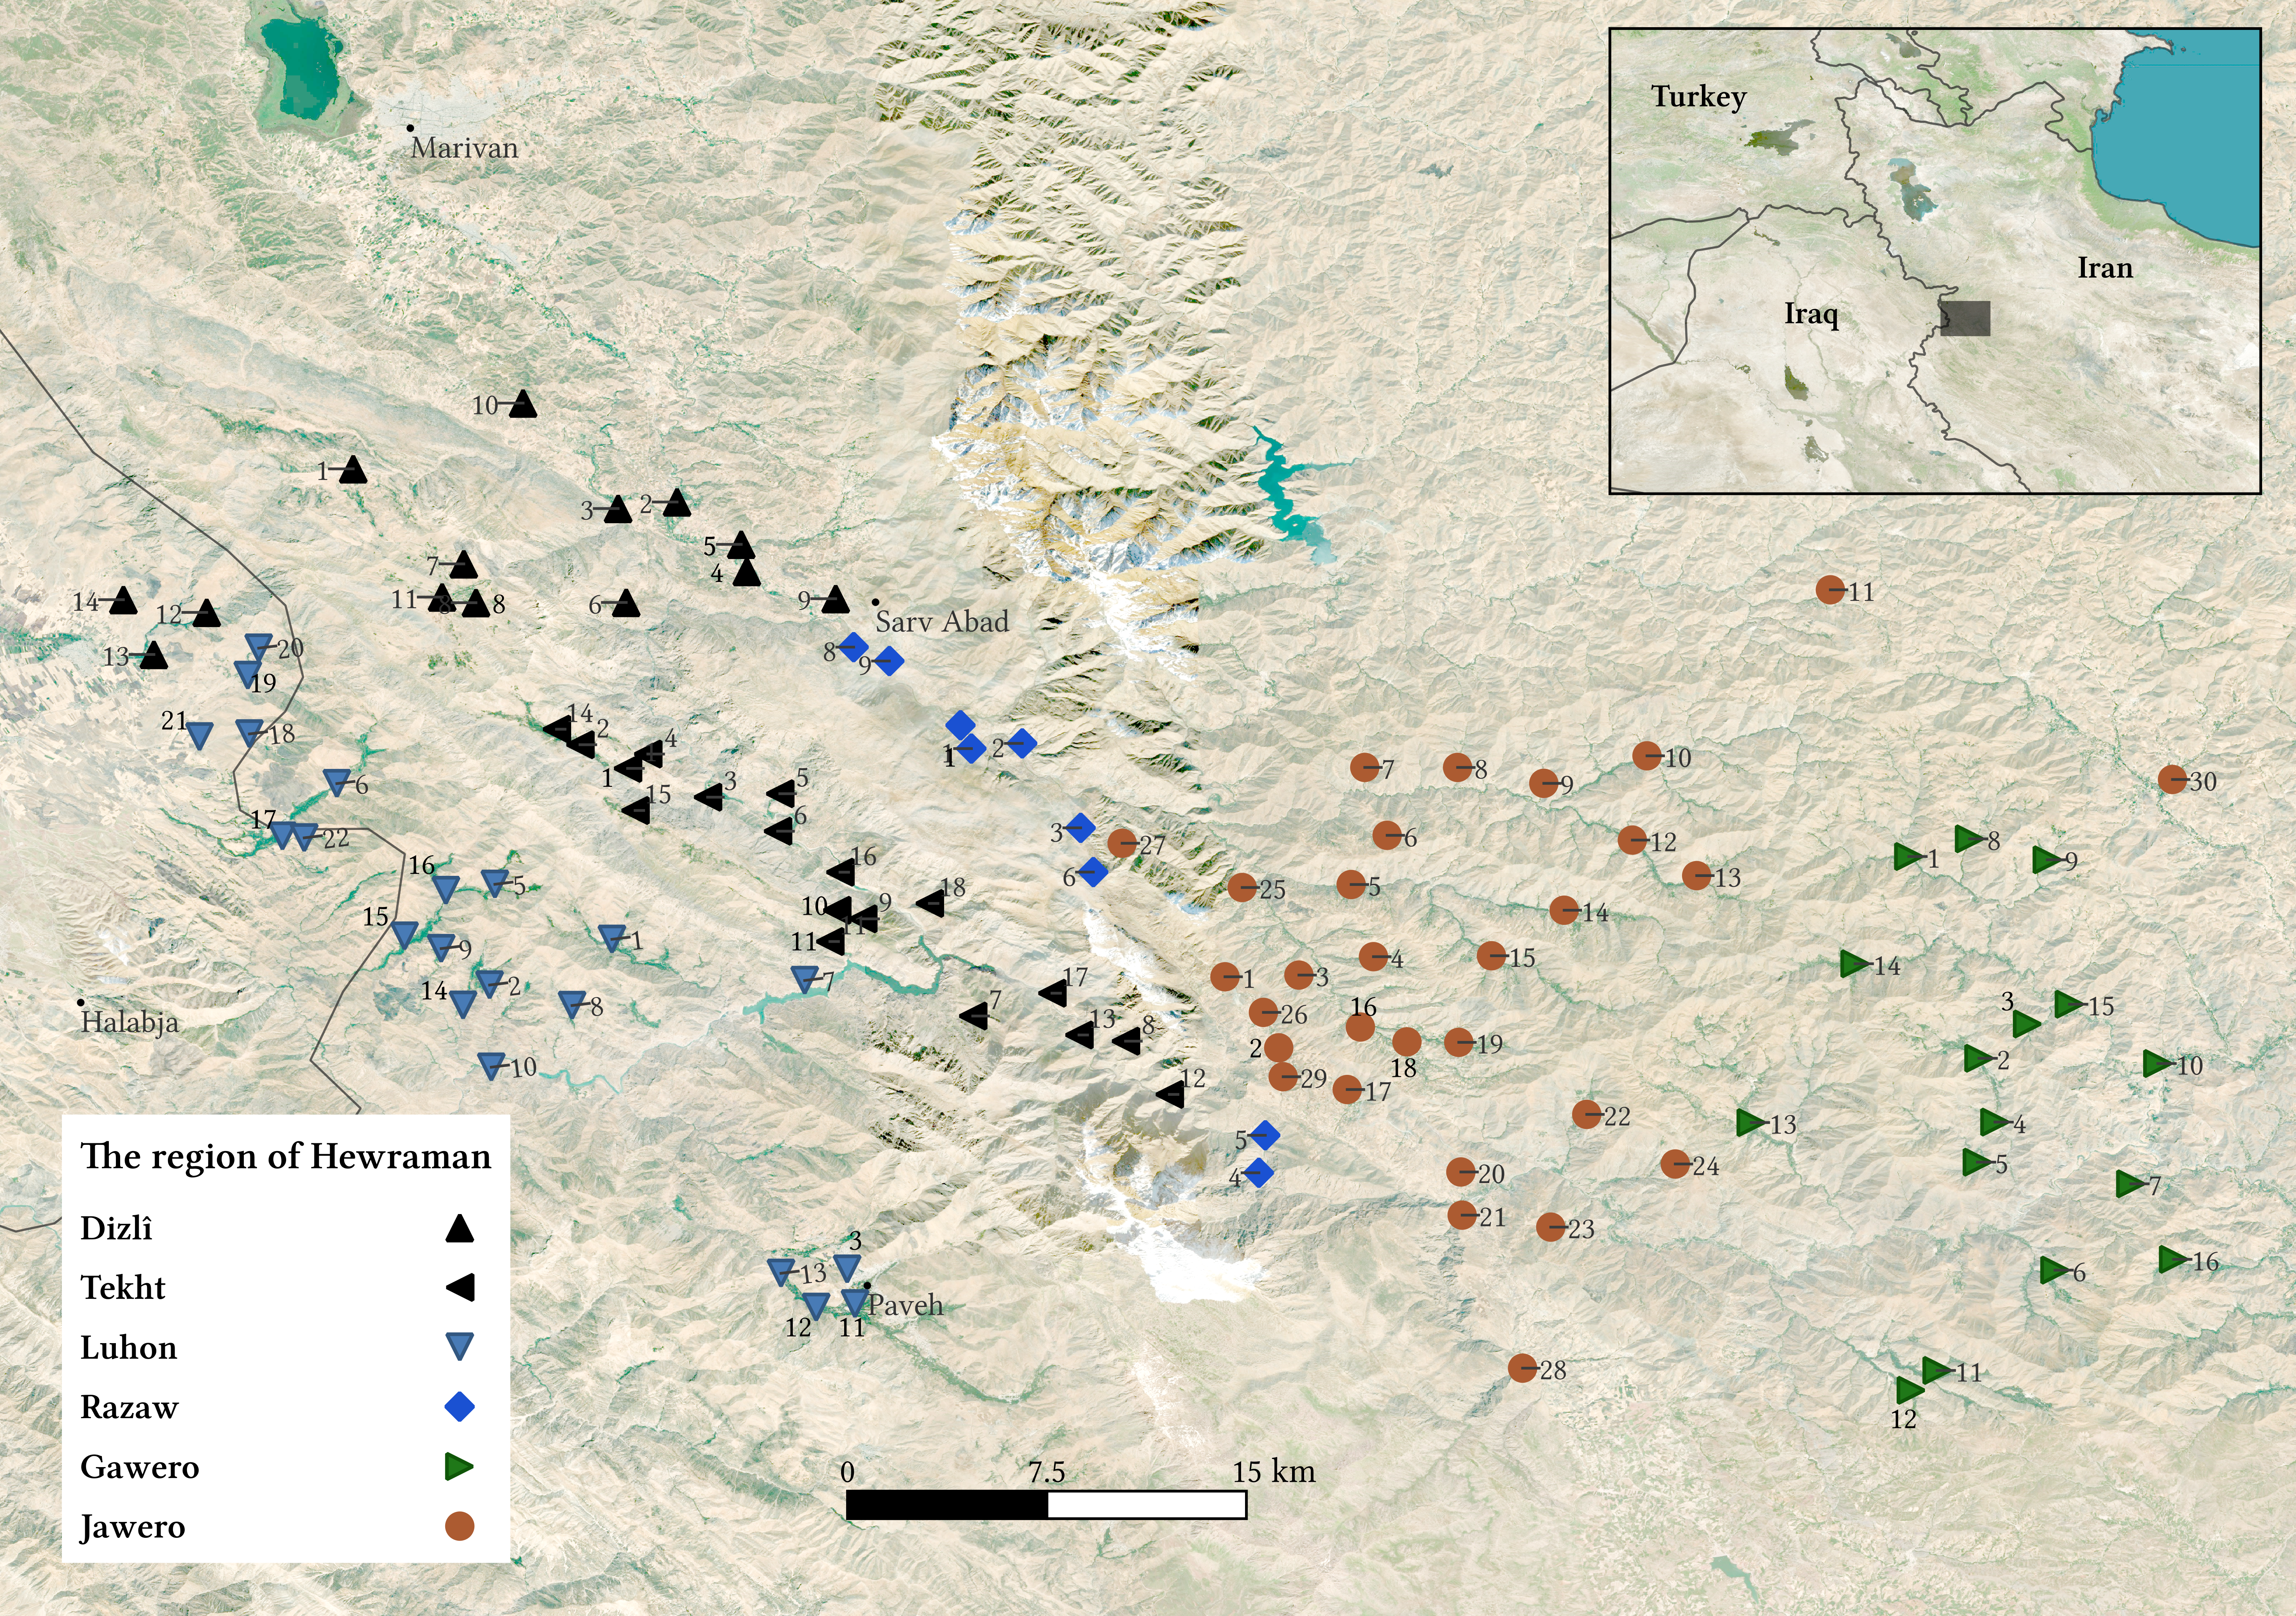
\includegraphics[width=\textwidth]{figures/Hewraman0107.png}
    \caption{The region of Hewraman and its divisions}
    \label{fig:hewmap}
    \end{figure}

There are no precise figures on the number of Hewramî\il{Hewramî} speakers. \citet{MacKenzie1987Avroman} puts the number of speakers at around 10,000. More recently, \citet{mohammadirad_language_2022} estimated the number of speakers to be about 120,000 in Kordestan province (western Iran) following a survey of linguistic distribution in the province. The population of Hewraman Tekht in the 2011 census was 2,761. The speakers refer to their language as \textit{Hewramî}, a term used by neighbouring Kurdish\il{Kurdish} speakers to refer to the Hewramî\il{Hewramî} vernacular. In addition, Hewramî\il{Hewramî}-speaking people self-identify as Kurds in a more socio-cultural and historical sense of the term Kurd, a sense which Kurds also employ to characterise Hewramî\il{Hewramî}s and Kurds alike.\footnote{See also \citet[25]{hassanpour_nationalism_1992}.} 

Although it is spoken by a small community, \citet[289]{hassanpour_nationalism_1992}{} reports that the Iranian government broadcast two-hour daily radio programmes in Hewramî\il{Hewramî} from 1977 to 1979. There was also broadcasting in Hewramî\il{Hewramî} after the Islamic revolution on Radio Sanandaj. These broadcasting programmes, however, did not result in the promotion of Hewramî\il{Hewramî}. Instead, the goal has been the political integration of the Hewramî\il{Hewramî}-speaking community. In Iraqi Kurdistan, broadcasting in Hewramî\il{Hewramî} has been boosted in recent years following the proliferation of TV channels. In neither of the sovereign states is Hewramî\il{Hewramî} promoted as an official language. More recently, the autonomous region of Iraqi Kurdistan has agreed that education be carried out in Hewramî\il{Hewramî} in localities with a significant Hewramî\il{Hewramî} population.

% and the propagation of the theory that the Hewramî community and Gorans were not Kurds
\section{The place of Hewramî\il{Hewramî} within Iranian dialectology} \label{sect:hew.ir.dialectology}
Hewramî\il{Hewramî} (ISO 639--3 hac) is a language that belongs to the Gorani\il{Gorani} language cluster of the Iranian languages (Indo-European: Iranian: Central Iranian: Northwestern Iranian: (Adharic:) Gorani\il{Gorani}: Hewramî\il{Hewramî}). 

Gorani\il{Gorani} varieties are scattered in the heart of Kurdish\il{Kurdish} parts of Iran and Iraq, shaded in Figure \ref{fig:goranidialects}. In Iran, there are Gorani\il{Gorani}-speaking communities south of the Hewraman region. The Gorani\il{Gorani} languages in Iraq are mostly placed to the west of the Hewraman region, from where they stretch as far as the Mosul plain to the north, where they are the vernacular of such communities as Kakaʼī, Šabak, Sarlī, or Bāĵaɫānī. 
\begin{figure}[htp]
    \centering
    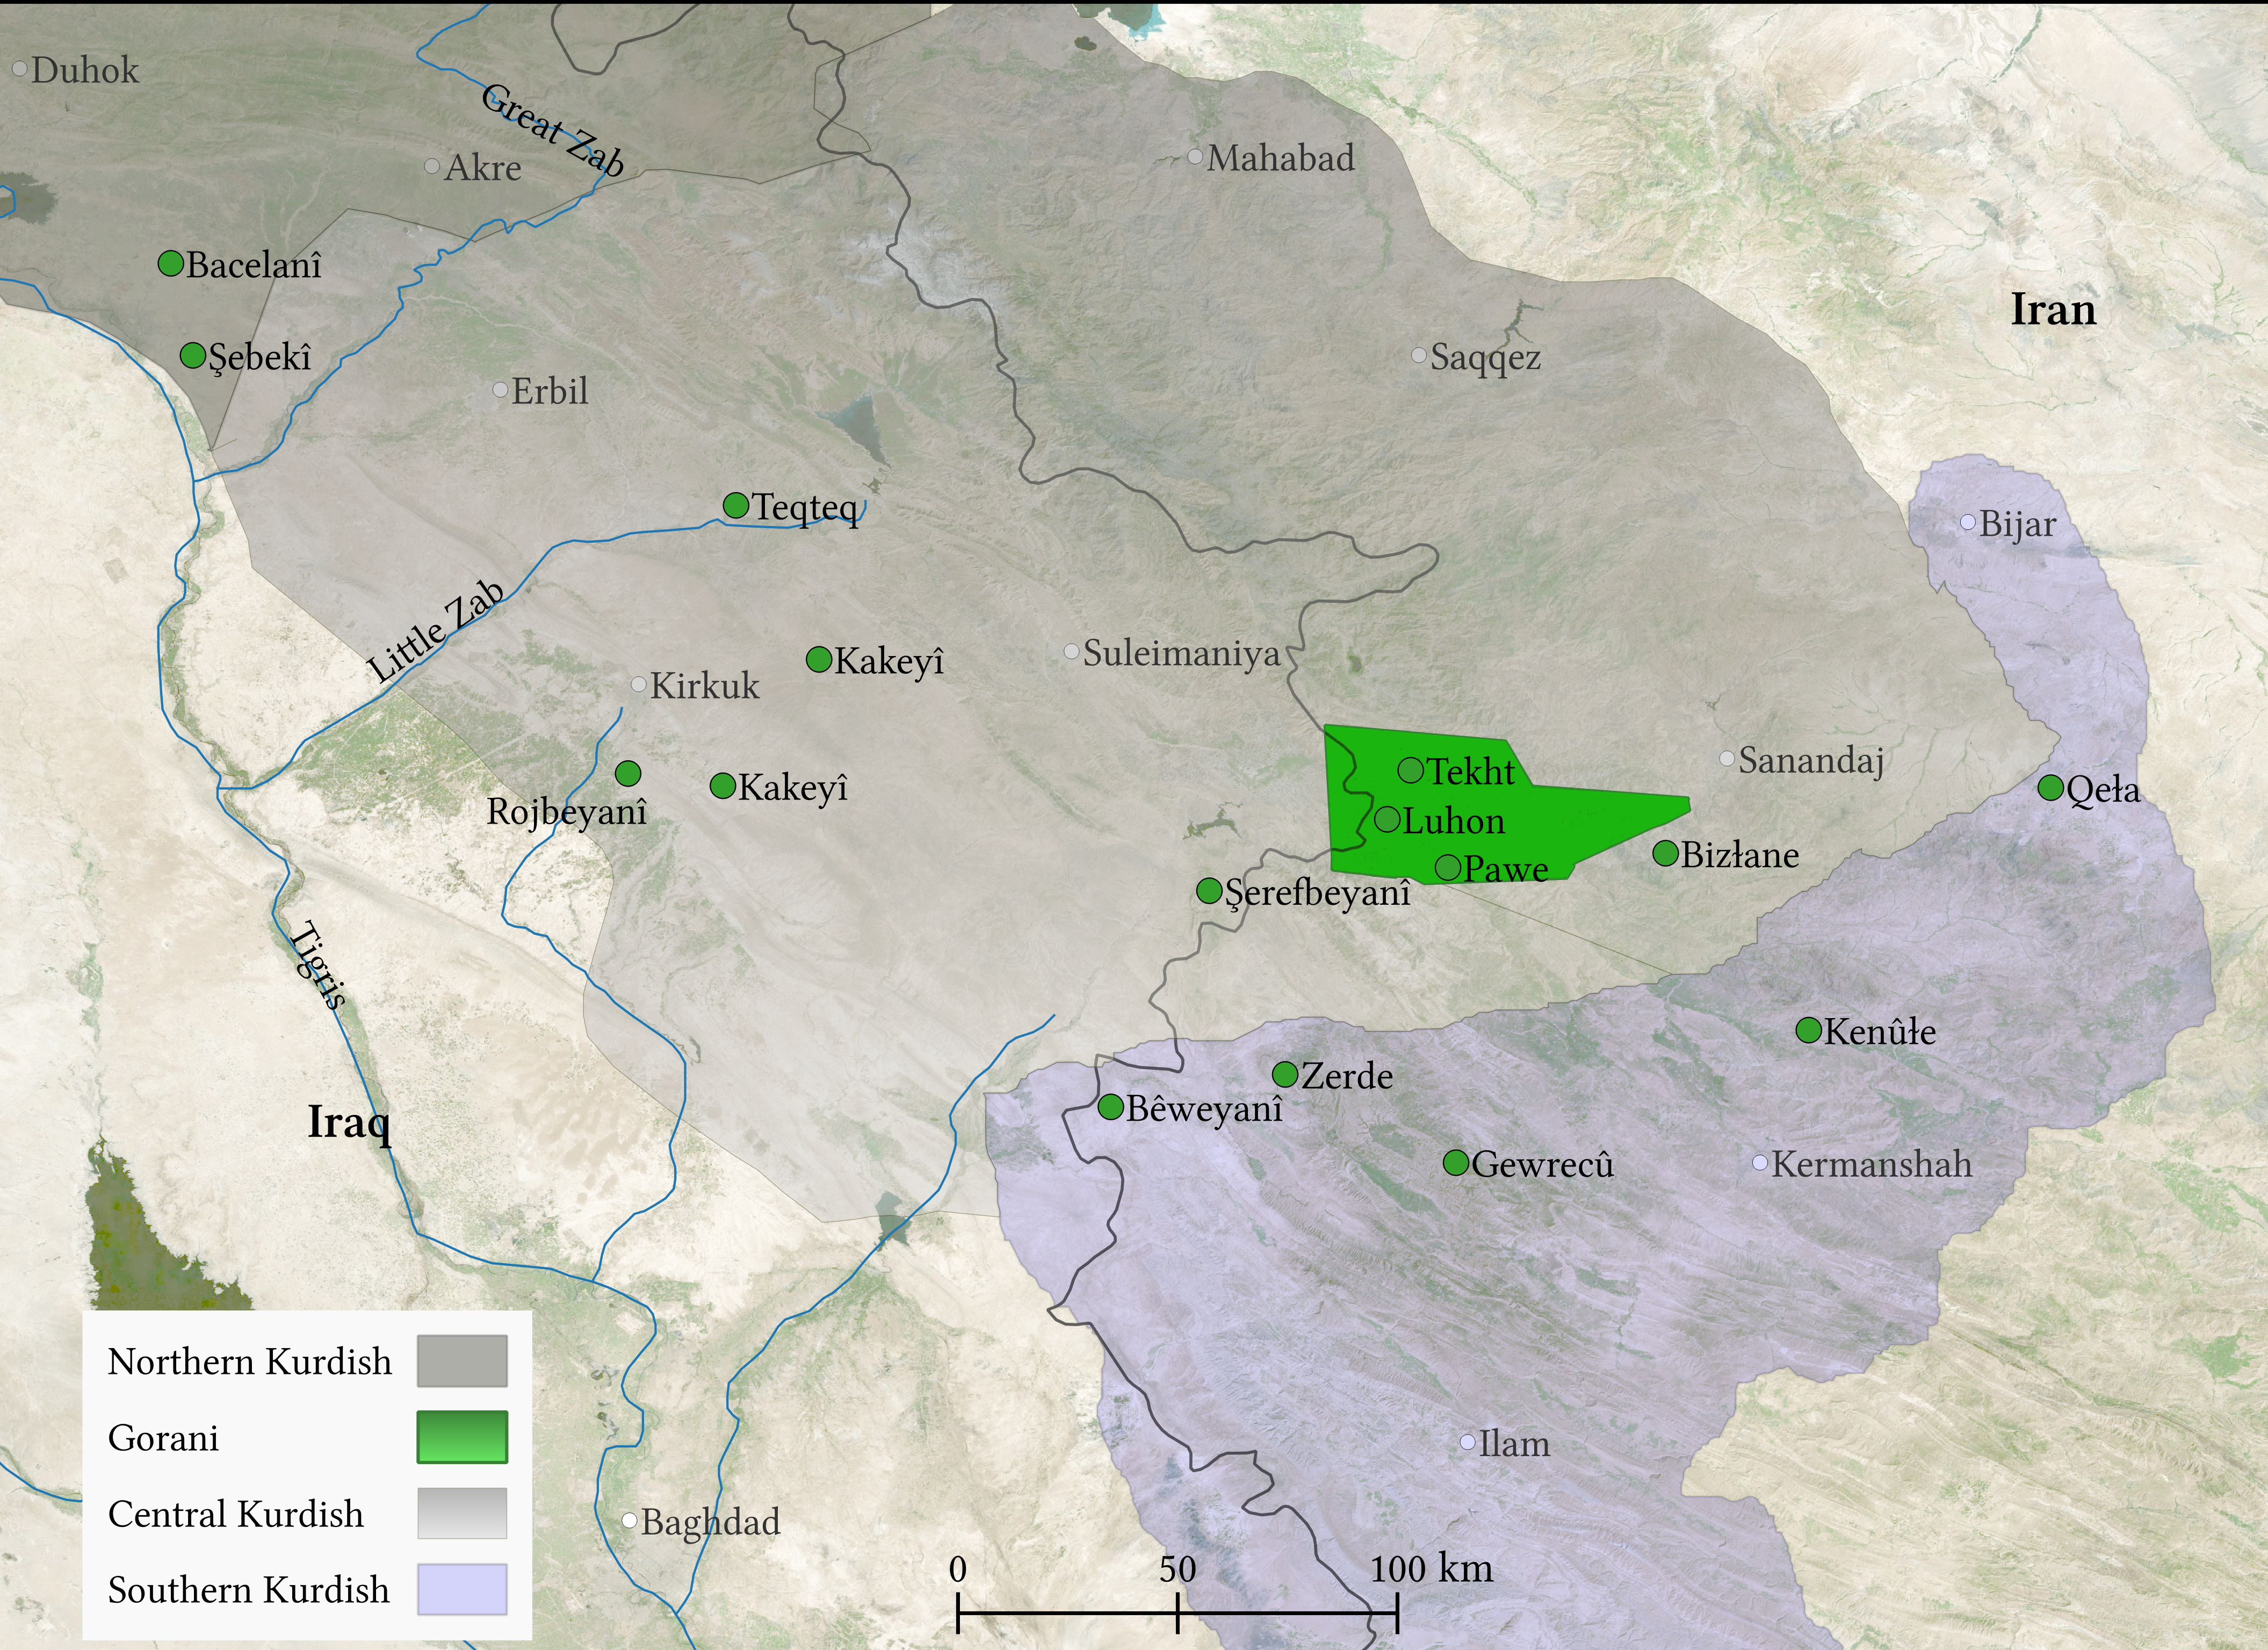
\includegraphics[width=\textwidth]{figures/Gorani dialects.png}
    \caption{Existing Gorani\il{Gorani} varieties}
    \label{fig:goranidialects}
\end{figure}

Gorani\il{Gorani} languages are characterised by preserving features dating back to the Old Iranian period. Within traditional Iranian philology, Gorani\il{Gorani} is considered a member of the Northwestern branch of Iranian languages along with Zazaki\il{Zazaki}, Taleshi\il{Taleshi}, and Kurdish\il{Kurdish}. Together with Zazaki\il{Zazaki}, Gorani\il{Gorani} varieties are shown to have preserved Northwestern phonological features par excellence \citep{paul_position_1998}.

Hewramî\il{Hewramî} is generally considered ``the best preserved and most archaic dialect" within the Gorani\il{Gorani} language cluster (see \citealt[4]{mackenzie_dialect_1966} and \citealt[]{MacKenzie1987Avroman}{}). The nominal morphology has preserved the fusional case\is{case}, gender\is{gender}, and number\is{number} affixes on nouns. In the verbal morphosyntax, ergativity is retained in verbal agreement and the nominal case marking\is{case marking}. Though note that 1st and 2nd person pronouns have lost case distinctions. Copula endings are distinguished for gender\is{gender} in the \textsc{3sg}. The progressive aspect is expressed by a constituent resembling an infinitive\is{infinitive} before the inflected form of the verb. Many of these features have been weakened or lost in the peripheral Gorani\il{Gorani} languages.

Varieties of Gorani\il{Gorani} were once spoken widely in the region. Gorani\il{Gorani} flourished as the literary language at the court of Ardalan principality (14th--19th centuries CE).\footnote{Gorani\il{Gorani} was also the court language of the neighbouring Baban principality, based in Suleimaniyya, up until the early 18th century when it was later replaced by Sorani Kurdish\il{Kurdish!Central} \citep{leezenberg_gorani_1992}.} Gorani\il{Gorani} also serves as the language of the religious texts of the heterodox Yarsan community in western Iran. 

Gorani\il{Gorani} varieties have been long in contact with vernaculars of Kurdish\il{Kurdish} and are assumed to predate Kurdish\il{Kurdish} in the region \citep{mackenzie_origins_1961}. The current distribution of varieties scattered across the Kurdish\il{Kurdish} zone gives evidence of a once-vibrant language, which gave way to Kurdish\il{Kurdish} over time (\citealt[]{mackenzie_dialect_1966}{}, \citealt[]{leezenberg_gorani_1992}{}). There are accounts of language shift to Kurdish\il{Kurdish} in some Gorani\il{Gorani} communities in the 19th and 20th centuries \citep[see][]{christensen_les_1921,kurdistani_mizgani_1930,leezenberg_gorani_1992, mahmoudveysi_meter_2016}{}{}. For example, \citet[3]{mahmoudveysi_meter_2016}{} reports that speakers of Bēwänījī, Rijābī, and Gähwāräī localities around Kerend (Iran), which were investigated by \citet[]{mann_mundarten_1930}{} as Gorani\il{Gorani} varieties, have now shifted to vernaculars of Southern Kurdish\il{Kurdish!Southern}.

 Recent scholarship has shown that the Gorani\il{Gorani} substrate within Kurdish and other local languages is most visible within the immediate Hewramî\il{Hewramî} zone of influence. \citegen{khan_language_2023} study of language contact in Sanandaj reveals that the impact of Hewramî\il{Hewramî} is far greater than Kurdish\il{Kurdish} on the Jewish Neo-Aramaic\il{Neo-Aramaic} dialect spoken there, suggesting that Hewramî\il{Hewramî} was once more widely spoken in this now dominantly Kurdish\il{Kurdish}-speaking town. A more recent study by the authors highlights the impact of Gorani\il{Gorani} on the Neo-Aramaic\il{Neo-Aramaic} dialect in Sanandaj and neighbouring Neo-Aramaic\il{Neo-Aramaic} varieties \citep{KhanMohammadirad+2024+171+198}. \citet[]{mohammadirad_gorani_nodate}{} is a case study of the Gorani\il{Gorani} substrate in the Southern varieties of Central Kurdish\il{Kurdish!Central}, e.g., CK Sanandaj, bordering the Hewramî\il{Hewramî} speech zone. In other publications, the author illustrates the Gorani\il{Gorani} substrate in the Southern varieties of Central Kurdish\il{Kurdish!Central} in the areas of bound inflectional morphology \citep[][]{mohammadirad_bound_nodate}{}{}, and word order\is{word order} \citep[][]{mohammadirad_zagros_nodate}{}{}. The picture that emerges from these most recent studies is that the morphosyntactic and phonological differences between the Northern varieties of Central Kurdish\il{Kurdish!Central} and Southern varieties of Central Kurdish\il{Kurdish!Central} can be understood by reference to a Gorani\il{Gorani}/Hewramî\il{Hewramî} substrate in the Southern varieties. 

 In recent years, a new line of scholarship has emerged that studies Gorani\il{Gorani}/Hewramî\il{Hewramî} varieties within the bigger Kurdish\il{Kurdish} dialectology e.g., \citet{opengin_pronominal_2022, mohammadirad_lenition_nodate}. The use of the term Kurdish\il{Kurdish}/Kurdic to refer to Gorani\il{Gorani}/Hewramî\il{Hewramî} varieties follows from the importance of Gorani\il{Gorani} in understanding the history of Kurdish\il{Kurdish} language and Gorani\il{Gorani} being part of Kurdish\il{Kurdish} in the larger socio-historical and cultural sense of the term Kurdish\il{Kurdish}. This latter sense is also reflected in the perceptual identity of Hewramî\il{Hewramî}/Gorani\il{Gorani} speakers. 

\section{Hewraman Tekht} \label{sect:hewramitext}
Tekht Hewramî\il{Hewramî!Tekht} is a variety of Hewramî\il{Hewramî}, spoken at the centre of the greater Hewraman region (see Figure \ref{fig:hewraman}). The term Tekht comes from the name of the region whose administrative centre is the city of Hewraman Tekht (Orāmān-e Takht). The town has a population of around 5,000. The inhabitants of the city are all Hewramî-speaking. The Hewraman region was registered as a cultural heritage by UNESCO in 2021.\footnote{\url{https : / / whc . unesco . org / en / list / 1647/}} This has led to an influx of tourists coming to the region both from within Iran and abroad and will undoubtedly have a bearing on the town's vernacular. 
\begin{figure}[htp]
    \centering
    \includegraphics[width=\textwidth]{figures/hewraman-village.jpg}
   \caption{Hewraman Tekht (photo credit: © Hamid Binaei Faa / UNESCO World Heritage Sites)}
    \label{fig:hewraman}
\end{figure}

The administrative region of Hewraman Tekht consists of 19 localities (see Figure \ref{fig:hewmap}). It is unclear if the vernacular of all these localities can be grouped under the Tekht variety, especially localities like Naw and Deɫemerz, located close to the Luhon and Jawero regions, respectively.

The inhabitants of the region are generally bilingual in Central Kurdish\il{Kurdish!Central}. This is most notably the case for men. Women over the age of 40 are usually monolingual in Hewramî\il{Hewramî}. The region's inhabitants also have some knowledge of Persian\il{Persian}, though it seems that competence in Persian\il{Persian} is higher among men than women. The situation for the younger generation is different since they all learn Persian\il{Persian} through schooling. It could be the case that the younger generation who has never left Hewraman does not speak any Kurdish\il{Kurdish} but knows Persian\il{Persian} through schooling. 

The inhabitants of Hewraman generally engage in an agropastoral lifestyle, which is semi-nomadic with vertical migration. During warm seasons, people migrate to the highlands, where they plant cereals, tend livestock, and migrate back to the lowlands during cold seasons. However, this lifestyle is waning, and the agropastoral lifestyle has given way to urbanism in Hewraman Tekht and increasingly in the surrounding villages. 

The Hewram\^i people are well known for their craftsmanship. Woodwork, stonework, and weaving shoes are still practised in Hewraman. The first two jobs are traditionally associated with men, while women generally weave shoes. The people of Hewraman traditionally engage in gardening. Mulberries and walnuts are common products in the region.

\section[The affiliation of Tekht Hewramî]{The affiliation of Tekht Hewramî\il{Hewramî!Tekht} and its status within Hewramî\il{Hewramî} dialectology} \label{sect:affiliation-hew}
Tekht Hewramî\il{Hewramî!Tekht} is one of the most conservative varieties of Hewramî. It is nearest in its morphosyntax to the Luhon variety studied by \citet{mackenzie_dialect_1966}. A general characteristic of Gorani\il{Gorani} varieties is that the more distance they are from the core mountainous Hewraman region, the less conservative they are. For instance, ergativity and nominal gender\is{gender} marking, belonging to the class of ``mature features\is{mature features}'' \citep{dahl_growth_2004}, tend to get lost in Gorani\il{Gorani} varieties outside Hewraman. 

Within Hewramî\il{Hewramî}, major varieties have notable morphosyntactic differences. While these differences await a thorough study, provisionally, the following features distinguish Tekht Hewramî\il{Hewramî!Tekht} from the neighbouring Luhon\il{Hewramî!Luhon} variety. 
The gender\is{gender} system of the two varieties exhibits some variation, as seen in the native lexicon below:

\TabPositions{2.5cm,5cm}
\ea
 Tekht H.\il{Hewramî!Tekht}\tab  Luhon H.\il{Hewramî!Luhon} \\
\textit{masaw} (\textsc{m})\tab  \textit{masawî} (\textsc{f})\tab  `fish' \\
\textit{asaw} (\textsc{m})\tab  \textit{asawî} (\textsc{f})\tab  `mill' \\
\textit{çiraw} (\textsc{m})\tab  \textit{çirawî} (\textsc{f})\tab  `lamp' \\
\z

In some loanwords\is{loanwords}, while the gender assignment\is{gender assignment} is identical, the endings differ across Tekht\il{Hewramî!Tekht} and Luhon\il{Hewramî!Luhon}. 
\TabPositions{2.5cm,5cm,8cm}
\ea
Tekht H.\il{Hewramî!Tekht}\tab  Luhon H.\il{Hewramî!Luhon} \\
\textit{hêɫeke}\tab  \textit{hêɫekî} \tab  `fine sieve' (\textsc{f}) \tab  cf. Turkish\il{Turkish} \textit{elek}\\
\z 

In nominal morphology, the two varieties differ in the use of the oblique case on past transitive subject (A-past) arguments. According to \citet[51]{mackenzie_dialect_1966}, in Luhon, the oblique case is limited to inanimate agents of past transitive verbs (A's). In Tekht, by contrast, oblique marking is additionally available for non-human animate A's (\ref{ex.animate-obl}) and human A's (\ref{ex.hum-obl}). In other words, the ergative case marking in Luhon is limited to the lowest agents in the animacy hierarchy. The Tekht variety retains an earlier stage of oblique marking on a broader range of agents, including human and non-human.
\ea 
\ea[]{
\textit{îse cawê kerdêne çêro.} \\ 
\gll îse \textbf{ caw(e)-ê} kerdê=ne çêr=o \\ 
 now road\textsc{-f.sg.obl} do\textsc{.pst.ptcp.f=cop.3sg.f:O} under\textsc{=post} \\ 
\glt `Now, the stone is laid under the road.' \hfill[ZP.53]
}
\ex[]{
\textit{marêwî gesta.} \\
\gll \textbf{mar-êw-î} gest-a \\
snake-\textsc{indf-m.sg.obl} bite.\textsc{pst-1sg:O} \\
\glt `A snake bit me.' \hfill[MP.09] \label{ex.animate-obl}
}
\ex[]{
\textit{pađşay desûriş dan be min.} \\ 
\gll \textbf{pađşa-î} desûr=iş da=n be min \\ 
 king\textsc{.m-sg.obl} order\textsc{.m=3sg:A} give\textsc{.pst.ptcp.m=cop.3sg.m:O} to \textsc{1sg} \\  
\glt `The king has ordered me [to do this].' \hfill[JP.209]\label{ex.hum-obl}
}
\z
\z

The Tekht variety\il{Hewramî!Tekht} preserves the gender\is{gender} distinction of predicative adjectives, e.g., in copula clauses. In the Luhon variety\il{Hewramî!Luhon}, by contrast, the feminine\is{feminine} form of the adjective is extended to the singular\is{singular} set. This is shown in (\ref{ex.wes.infl1}) for the inflection of \textit{weş} `well'.
\ea \label{ex.wes.infl1}
Luhon H.\il{Hewramî!Luhon}\tab  Tekht H.\il{Hewramî!Tekht} \tab   \\
 \multirow{2}{*}{\textit{weşe=na}}\tab  \textit{weş=na}\tab  `I (\textsc{m}) am well.' \\
\tab  \textit{weşe=na}\tab  `I (\textsc{f}) am well.'\\
 \multirow{2}{*}{\textit{weşe=nî}}\tab  \textit{weş=nî}\tab  `You (\textsc{m}) are well.' \\
\tab   \textit{weşe=nî}\tab  `You (\textsc{f}) are well.'\\
\z 

The two varieties exhibit differences in the stem formation of several verbs. 
\TabPositions{1.5cm,4cm,6cm,8cm}
\ea
Tekht H.\il{Hewramî!Tekht} \tab  \tab Luhon H.\il{Hewramî!Luhon}\\
\textsc{prs} \tab  \textsc{pst} \tab  \textsc{prs} \tab  \textsc{pst} \\
\textit{wen-}\tab  \textit{wena-}\tab  \textit{wan-}\tab  \textit{wana-}\tab  `read'\\
\textit{piseř-} \tab  \textit{piseřa-} \tab \textit{ seř-} \tab  \textit{seřa-} \tab  `wipe' \\
\textit{cen-}\tab  \textit{cena-}\tab  \textit{incen-}\tab  \textit{incena-} \tab  `mince' \\
\textit{biřfan-}\tab  \textit{biřfana-}\tab \textit{ řfan-}\tab  \textit{řfana-}\tab  `abduct' \\
\z 

Both varieties employ preverbal TAM prefixes (i.e., indicative and subjunctive prefixes) to a limited extent. Phonological factors condition the occurrence of these prefixes, e.g., before vowel-initial verbs in both varieties. However, Luhon H.\il{Hewramî!Luhon} tends to use these prefixes with more verbs; see (\ref{ex.ind-sbjv-difference}). For example, w-initial verbs tend to take the indicative prefix in Luhon\il{Hewramî!Luhon}, but not in Tekht\il{Hewramî!Tekht} (See \citealt[]{karim_imperfective_inreview}{, for explanation}).

\TabPositions{2.5cm,5cm}
\ea \label{ex.ind-sbjv-difference}
Tekht H.\il{Hewramî!Tekht}\tab  Luhon H.\il{Hewramî!Luhon}\\
\textit{wan-o} \tab  \textit{mi-wan-o} \tab  `he/she reads'  \\
\textit{wer-o} \tab  \textit{(mi)-wer-o} \tab  `he/she eats' \\
\textit{taw-o} \tab  \textit{mi-taw-o} \tab  `he/she can' \\
\textit{zan-o} \tab  \textit{mi-zan-o}\tab  `he/she knows' \\
\textit{\v{r}em-o} \tab  \textit{mi-\v{r}em-o}\tab  `he/she runs' \\
\z

\section{Earlier research} \label{sect:lit.gorani}

Gorani\il{Gorani} languages, among them the Hewramî\il{Hewramî} varieties especially, have long intrigued philologists and linguists alike. A first major -- and often unnoticed -- monograph-length study on a variety of Hewramî\il{Hewramî} was a descriptive grammar of Tekht Hewramî\il{Hewramî!Tekht} and the Pawe\il{Hewramî!Pawe} dialect (spoken in the northeast of Kermanshah in the city of Pawe) by \citet{christensen_les_1921}. This grammar resulted from a field trip to Sanandaj and Hewraman by Åge Meyer Benedictsen in 1901. The Hewramî\il{Hewramî} description comes from a collection of seven texts, four of which were collected from a young speaker of Ruwar dialect (P. Rūbār), whom Benedictsen met in Sanandaj. The remaining three texts were collected in Hewraman, in the village of Nawe S\^ute, which I have been unable to locate on the map. The Pawe material features one text and four poems. 

A second major work on Gorani\il{Gorani} varieties was carried out by \citet{mann_mundarten_1930}. The book contains chapter-long descriptions of eight Gorani\il{Gorani} varieties, including Kanduali, Auramani, Bajalani, Biwaniji, Gahwarai, Rijabi, Sayyidi, and Zardai. Among these, only Kandulai has been described in detail. Little grammatical description is offered for the rest of the varieties, and the respective sections consist mainly of lexicon and a few texts. The Auramani sketch deals with the linguistic analysis of proper Hewramî\il{Hewramî}, though, as \citet{mackenzie_dialect_1966} notes, it is not evident which dialect of Hewramî\il{Hewramî} is investigated here. 

The best-known grammar of Hewramî\il{Hewramî} is \citegen{mackenzie_dialect_1966} description of the Luhon\il{Hewramî!Luhon} dialect of Hewramî. The monograph is based on the speech of a single male Kurdish\il{Kurdish}-Hewramî\il{Hewramî} bilingual whom MacKenzie met in London. The grammar is detailed and remains the only reliable description of a variety of Hewramî\il{Hewramî} ever since. Nonetheless, it is brief and economical. Indeed, the book mainly covers morphology, perhaps in line with the tradition of grammar writing at the time. Less coverage has been given to phonology and especially syntax. 

In recent years, several scholars have devoted themselves to describing the most endangered varieties of Gorani\il{Gorani}, situated outside Hewraman and considered peripheral Gorani varieties. This has resulted in the publication of two sketch grammars of the peripheral Gorani varieties of Gewrecû\il{Gorani!Gewrecû} \citep{mahmoudveysi_gorani_2012} and Zerde\il{Gorani!Zerde} \citep{mahmoudveysi_gorani_2013}, spoken in western Iran. \citet{mahmoudveysi_hawrami_2018} offer a short grammatical description of the Hewramî dialect of Pawe\il{Hewramî!Pawe}. The authors have now embarked on preparing a grammatical description of the Shabaki\il{Gorani!Shabaki} dialect of Gorani spoken in the Mosul Plains.

Despite the recent rising interest in Gorani\il{Gorani} varieties, \citegen{mackenzie_dialect_1966} descriptive grammar is the only standard description of a Hewramî\il{Hewramî} variety to date. Other varieties of Hewramî\il{Hewramî} remain largely under-investigated. This book aims to provide a detailed grammatical description of the Tekht variety of Hewram\^i\il{Hewramî!Tekht}, which, as seen in \S\ref{sect:affiliation-hew}, differs in many respects from the more southern Luhon variety. The grammar is based on field recordings I collected over the course of several field trips to the Hewraman region over the past seven years. It provides a detailed account of the phonetics, phonology, morphology, syntax and lexicon of Hewramî, grounded in current linguistic methods. Despite what is often assumed, there is a high degree of dialectal variation within Hewramî\il{Hewramî} varieties. Indeed, it is unclear whether the vernaculars of Dizlî and Şamyan belong to any known three varieties of Hewramî\il{Hewramî}. Likewise, the morphosyntactic features of the Jawaro variety remain largely unknown to scholars working on Hewramî\il{Hewramî} dialectology. It is hoped that the current monograph will encourage scholars to produce comprehensive descriptions of the remaining Hewramî\il{Hewramî} varieties.

\section{Fieldwork behind this study} \label{sect:fieldwork}

The material for this book was mainly gathered during various rounds of fieldwork conducted in Hewraman Tekht between March 2016 and August 2023. I visited the region for the first time in March 2016 and conducted a pilot linguistic fieldwork. On this first field trip, my goal was mainly to get familiar with the speech community and get an idea of patterns of language use on a daily basis. I recorded spontaneous speech and dialogues, and conducted a few elicitation tasks, primarily focusing on verb conjugation. A recording I collected on this trip appears as a glossed text in \citegen[557--564]{khan_language_2023} study of language contact in Sanandaj. 

The second field trip took place in June and July 2017. This trip was conducted as part of my PhD dissertation on pronominal clitics in Western Iranian languages. During this trip, I conducted elicitation tasks using visual stimuli and a questionnaire with native speakers from Hewraman Tekht. In addition, I recorded some spontaneous spoken data and recorded a narration of the \textit{Pear story}. The elicited and spontaneous data collected in this trip formed the basis for the study of argument indexing and syntax of pronominal clitics in Tekht Hewramî\il{Hewramî!Tekht} \citep[see][365--372]{mohammadirad_pronominal_2020}{}{}, within the context of Western Iranian languages. 

The material from these two trips, additional elicited grammar surveys carried out with Hewramî\il{Hewramî} speakers, and further recordings served as the basis for the description of linguistic features of Tekht Hewramî\il{Hewramî!Tekht} in \citegen{khan_language_2023} detailed study of language contact in Sanandaj entitled: \textit{Language contact in Sanandaj: A study of the impact of Iranian on Neo-Aramaic}. The documentation of Hewramî began to take shape during the work with Geoffrey Khan on the mentioned book between 2020 and 2023.  

The linguistic material for this book comes principally from a field trip to the region in August 2022. During that field trip, which lasted three weeks, I contacted the locals in Hewramî\il{Hewramî}, which greatly facilitated fieldwork and contact with the inhabitants. I made recordings of 15 narratives. The recordings were made using a Zoom H5 Handy Recorder, which produced audio files in WAV format. I conducted my fieldwork mostly in Hewraman Tekht but also visited Serû Pîrî (a village north of Hewraman) and Benen (the summer habitat for the inhabitants of Hewraman Tekht, located in the highlands). During this fieldwork, I transcribed most of the recordings and double-checked my interpretation of recordings with my native assistant, Amir, to ensure that the correct interpretation had been achieved. In addition, I carried out many elicited grammar surveys (including a questionnaire) with Amir and, occasionally, with a few other people in Hewraman Tekht. The questionnaire was developed within the framework of the project “A Linguistic History of Minorities in the Near East” at the University of Cambridge for studying phonological, morphosyntactic, and lexical variation within Kurdic.\footnote{\url{https://www.ames.cam.ac.uk/research/project/echoes-vanishing-voices-mountains-linguistic-history-minorities-near-east}} The 15 narratives collected in this trip were transcribed and translated and later fully glossed as a text corpus volume representing Hewramî oral narratives (see \citealt{mohammadirad_speking_the_past} for details).

The fourth field trip took place in July 2023. On this trip, I mainly conducted elicitation tasks on issues I encountered while preparing a first draft of the current grammar. Additionally, I compiled the verb list presented in Appendix \ref{verb_list} and collected more recordings in Hewraman Tekht. During this trip, I collected further recordings of spontaneous speech in Hewraman Tekht, Serû Pîrî, and Bennen. This trip allowed me to travel to the nearby villages and get a first impression of linguistic diversity within the localities in which Tekht Hewramî\il{Hewramî!Tekht} is spoken. I was lucky to meet two competent storytellers in Nwên (one of whom was originally from Silên), who narrated some 25 spoken narratives characteristic of the folkloristic tradition in Hewraman. These narratives, as well as a few additional tales that I gathered in Hewraman Tekht in July 2023, constitute a collection of tales, a comprehensive processing of which is planned as a projected publication \citep{mohammadirad_folktale_inprep}. In discussing the linguistic features of Tekht Hewramî\il{Hewramî!Tekht}, I sometimes draw on the folkloristic material just discussed (see \S\ref{sect:folktale-corpus}) to back up the description of Hewramî\il{Hewramî} features. Still, the main grammatical analysis is based on the glossed text corpus in \citet{mohammadirad_speking_the_past}. 

\section{Main text corpus} \label{sect:corpus.hewrami-text}

The 15 narratives collected in August 2022 (see the previous section) comprise the main corpus behind the current book. These narratives yield a total of 96 minutes of running speech. The recordings have been time-aligned with translation using the annotation software ELAN. The recordings, along with the ELAN files, and time-aligned texts, have been archived on the open-access platform Zenodo (see \citealt{mohammadirad_2025_15419952}), and can be found at \url{https://zenodo.org/records/15419952}.

The recorded texts belong to different supposed genres: folktales, local anecdotes, myths, oral history of the region, and autobiographies. The resulting texts form the Tekht Hewramî\il{Hewramî!Tekht} database and are a touchstone for the grammatical description and lexicon. The text corpus behind this study has been entirely glossed in FLEx, from which the glossed texts were converted into the specific formatting for linguistic examples required by Language Science Press in \LaTeX, using a Python script. The glossaries at the end of the book were drawn from the TeX file using additional Python scripts. 

The narrators who recounted the narratives were all over 60 years old at the time of recording. In many ways, then, this descriptive grammar is indicative of the language as spoken by the older generation. Nonetheless, in a few cases, the grammar highlights the generational difference in language use. As for the linguistic profile of the narrators, except for the narrator of the text JE, who is a monolingual, the rest exhibit some bilingualism in Kurdish\il{Kurdish}. These speakers have a weak bilingualism pattern, with Hewramî\il{Hewramî} as their dominant language and Kurdish\il{Kurdish} as less dominant. In addition, some of these narrators showed weak competence in Persian\il{Persian}.

\begin{table}[t]
\caption{The main text corpus \citep[]{mohammadirad_speking_the_past}}
\label{tab:texts}
    \centering
    \small
\begin{tabularx}{\textwidth}{QlQr}
    \lsptoprule
       \textsc{title} & \textsc{id} &\textsc{topic} \\
	\midrule
		\textit{zaroɫe û bizê} `The baby and the goat' & ZB & Local anecdote/myth about an abandoned baby  \\
       \textit{zaroɫe û qiřolû darî} `The baby and the tree hollow' & ZQ &Local anecdote/myth about an abandoned baby  \\
       \textit{herbene} `The donkey keeper' & HB & Local anecdote/myth about a talking donkey \\
        \textit{peɫê merekuř} `A swarm of grasshoppers' & PM  &Local anecdote/myth, grasshoppers \\
        \textit{derde gulî} `Leprosy' & DG & Local anecdote/myth about a man suffering from leprosy \\
        \textit{Şêx ʕumer û Cafir san} `Sheikh Omar and Jafir San' & ŞC & Local anecdote about recent history  \\
        \textit{duwê padşε} `Two kings' & DP  & Oral history, two kings claiming Hewraman \\
        \textit{jîwayû Pîr Şelîyarî} `Pir Shaliyar’s life' & JP  & Oral history, hagiography  \\
        \textit{zemawinew Pîr Şalîyarî} `Pir Shaliyar’s wedding' & ZP & Oral history, hagiography \\
        \textit{babaw Pîr Şalîyarî} `Pir Shaliyar’s grandfather' & BP & Oral history, hagiography \\
        \textit{kuřû şuwaney} `The shepherd’s son' & KŞ  & Folktale \\
        \textit{jîwayû Heyasî} `Hayas’s life' & JH  & Folktale \\
        \textit{řisûmatû ewsayma} `Our past traditions' & RE & Recollections of traditional life \\
        \textit{jîwayû ewsayma} `Our past life'  & JE & Recollections of traditional life, autobiography \\
       \textit{jîwayû min} `My life'  & JM  & autobiography \\
    \lspbottomrule
\end{tabularx}
\end{table}


The 15 narratives consist of approximately 10,000 words. Table \ref{tab:texts} lists the titles of the texts and their identifier codes in \citegen[]{mohammadirad_speking_the_past} volume. The examples taken from the latter volume are cited in the grammar using the initials of the texts along with an identifier number corresponding to the numbered annotation units--typically a sentence or a clause. For instance, ZB.20 corresponds to sentence number 20 in the ZB text. This guides the readers to the larger linguistic context from which the examples are taken.


There are some glossing and translation conventions worthy of noice. Object language examples are presented in two versions, an orthographic one that corresponds to actual surface realisations, and the morphologically segmented version, which contains representations of the morphemes that are closer to their assumed underlying forms. Example (\ref{ex.awunderlyin}) illustrates how the surface form \textit{awekê} `the water' in the orthographic version can be segmented at the underlying representation, while the second line in example (\ref{ex.kisunderlyin}) illustrates the underlying analysis for \textit{winû} `blood of' and \textit{kîseɫê} `tortoise (\textsc{f.sg.obl})' in the orthographic version. 

\ea \label{ex.awunderlyin} 
\textit{awekê biřo.} \\ 
\gll aw(î)-ekê biř-o \\ 
 water\textsc{.f-def.f.sg} cut\textsc{.prs.ind-3sg:A} \\ 
\glt `He cut off the water supply.' \hfill[DP.34]
\z 

\ea \label{ex.kisunderlyin}
\textit{winû kîseɫê sawî be...} \\ 
\gll win(î)-û kîseɫ(î)-ê s\'aw-î be \\
 blood\textsc{.f-ez.gen} tortoise\textsc{.f-obl.f} rub\textsc{.prs.sbjv-2sg:A} to \\ 
\glt `You may rub tortoise's blood on ...'  \hfill[DG.47]
\z 

A feature of Hewramî narratives is the frequent use of the present tense as the narrative tense to recount past events (see \S\ref{sect:narrativeprs}). Consequently, all the tales and narratives in \citet[]{mohammadirad_speking_the_past,mohammadirad_folktale_inprep} --- which are the source for linguistic examples in the current book --- have been translated into the past tense, including in cases where the narrative present is used to describe past time events (see \ref{ex.awunderlyin} for an example). Readers are encouraged to keep this in mind when interpreting the examples. 

In the translation of linguistic examples, square brackets indicate words and meanings that are implicit or not stated in the text, while round brackets clarify the reference of participants in the text, see \REF{ex.trans}.

\newpage
\ea \label{ex.trans}
\textit{maço, `nezanam.'}\\ 
\gll m-aç-o ne-zana=m\\ 
 \textsc{ind-}say\textsc{.prs-3sg:A} \textsc{neg-}know\textsc{.pst=1sg:A}\\ 
\glt `He (the man) said, `I didn't understand [his point].' \hfill[JH.26]
\z 

\section{Folktale corpus} \label{sect:folktale-corpus}
As briefly discussed in \S\ref{sect:corpus.hewrami-text}, the morphosyntactic description of Hewramî\il{Hewramî} is further backed up by additional folktales which I gathered at Nwên and Hewraman Tekht in August 2023. These folktales provide a rich source for studying the folkloristic tradition of Hewraman. Once fully processed, they will be published as a collection of folktales from Hewraman. For the current grammar, I have occasionally included example sentences from these tales in the main text. All the examples in the book from the folktale collection come with the initials of the tales and an identifier number, which refers to the place where the examples have been cited within the mentioned tale.

The folktale collection consists of 31 tales, totalling around 25,000 words. Here, it suffices to name each narrative with its initials, with a detailed description awaiting a projected publication of these tales \citep{mohammadirad_folktale_inprep}. \\
\\
1. \textit{mûsa û řuwase} (MR) `Moses and the fox' \\
2. \textit{mama mama} (MM) `Mama mama' \\
3. \textit{pîrejenî û kitê} (PK) `The old woman and the cat' \\
4. \textit{dêđê û çwar kinaçê} (ÇK) `The stepmother and four girls' \\
5. \textit{jenê fêlebaze} (JF) `A cunning wife' \\
6. \textit{jenî û lîrewireş} (JL) `The woman and the lira-seller' \\
7. \textit{wiɫkɫe} (WL) `Wilkle' \\
8. \textit{hacî û jenekêş} (JC) `Haji and his wife' \\
9. \textit{şaw mara û şaw melekuřa} (ŞŞ) `The king of snakes and the king of grasshoppers' \\
10. \textit{jenî û ħewt weywê} (HW) `A woman and seven daughters-in-law' \\
11. \textit{patşa û pîrî} (PP) `The king and the old man' \\
12. \textit{kuře keçeɫe} (KK) `The bald boy' \\
13. \textit{hêyasî jîr} (HJ) `Heyas the Wise' \\
14. \textit{siɫtan mehmûđ û heyasî jîr} (SH) `Sultan Mahmoud and Heyas the Wise' \\
15. \textit{meɫik ehmeđ} (ME) `Malek Ahmad' \\
16. \textit{Kinaçêw Taɫî meẍrêbî} (KT) `The daughter of Tal from Maghreb' \\
17. \textit{mar û peyxwmer} (MP) `The snake and the Prophet' \\
18. \textit{meɫa yoso û meɫa xiđir} (YX) `Mullah Yoso and Mullah Khidr' \\
19. \textit{şê bayzîdî boystamî} (BB) `Sheikh Bayzid Bostami' \\
20. \textit{çil paɫewanê û hezretû ʕelî} (ÇH) `Forty warriors and His Highness Ali' \\
21. \textit{pađşa û wezîr} (PW) `The king and the vizier' \\
22. \textit{duwê birayê} (DB) `Two brothers' \\
23. \textit{meɫa xiđir û şûwane} (XŞ) `Mullah Khidr and the shepherd' \\
24. \textit{xiđre xuɫekêş} (XX) `Khidr the Soil Carrier' \\
25. \textit{ehmeđe dize} (ED) `Ahmad the Thief' \\
26. \textit{şa ʕebas} (ŞE) `Shah Abbas' \\
27. \textit{sîyawehş û keyxesrew} (SK) `Siyawahsh and Keykhosrow' \\
28. \textit{hezretû mûsay û fêrʕon} (MF) `Moses and Pharaoh' \\
29. \textit{hacî mehmûđ û řozgarya} (HM) `Haji Mahmoud and the Rozgaris' \\
30. \textit{bêjen û menîje} (BM) `Bezhan and Manizha' \\
31. \textit{heyas û siɫtan mehmûyî} (HS) `Heyas and Sultan Mahmoud' \\


\end{sloppypar}
